\begin{tikzpicture}[x=1cm,y=1cm,>=Stealth,font=\small,
  cell/.style={draw,fill=white,minimum height=.48cm,align=center},
  fat/.style={->,line width=1.2pt},
  hollow/.style={->,draw=black!70,line width=3pt}]
  \path[use as bounding box] (0,0) rectangle (15.55,8.65);
  \node[cell,fill=blue!10,minimum width=1.30cm,minimum height=1.03cm] (st-data) at (.75,7.58) {真实\\数据};
  \node[cell,minimum width=2.80cm,minimum height=.65cm,font=\bfseries] (st-envtitle) at (3.35,7.84) {环境};
  \draw[hollow] (st-data.east) -- (st-envtitle.west);
  \draw[thick] (1.78,3.72) rectangle (4.92,7.32);
  \foreach \name/\y/\txt in {users/6.91/用户,messages/6.21/消息,network/5.51/网络}
    \node[cell,minimum width=2.72cm] (st-\name) at (3.35,\y) {\txt};
  \node[inner sep=0pt] at (3.35,4.47)
    {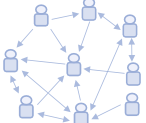
\includegraphics[height=1.45cm]{figures_zh/ch17/struct_network}};
  \node[text=red!75!black,font=\bfseries] at (5.22,8.44) {感知};
  \draw[hollow] (5.18,7.22) -- (5.72,7.22);
  \draw[thick] (6.05,3.95) rectangle (12.53,8.18);
  \node[cell,minimum width=2.15cm,minimum height=.63cm] (st-prompt) at (8.20,7.62) {提示设计};
  \node[cell,minimum width=2.15cm,minimum height=.63cm] (st-tuning) at (10.55,7.62) {调优};
  \node[text=red!75!black,font=\bfseries,align=center] at (13.65,7.66) {异质性\\与个性化};
  \node[draw=blue!50!black,fill=blue!10,minimum width=5.55cm,minimum height=.85cm,font=\bfseries]
    at (9.26,6.48) {大语言模型驱动的智能体};
  \draw[rounded corners=9pt,thick] (6.36,4.18) rectangle (12.08,5.72);
  \node[fill=blue!12,rounded corners=3pt,minimum width=3.35cm,minimum height=.57cm] at (9.28,5.77) {内部状态};
  \node[inner sep=0pt] at (7.13,5.77) {
\includegraphics[height=.83cm]{figures_zh/ch17/struct_person}};
  \foreach \x/\txt in {7.42/情绪,9.30/态度,11.13/其他}
    \node[cell,minimum width=1.53cm,minimum height=.57cm] at (\x,4.74) {\txt};
  \draw[hollow] (9.25,3.84) -- (9.25,3.22);
  \node[text=red!75!black,font=\fontsize{8.5}{10}\selectfont\bfseries] at (10.99,3.51) {推理与决策};
  \node[cell,fill=blue!9,minimum width=5.55cm,minimum height=.68cm,font=\bfseries] (st-gen) at (9.25,2.83) {生成模块};
  \node[cell,minimum width=1.90cm,minimum height=.63cm,text=blue!45,font=\bfseries] (st-cond) at (3.35,2.81) {条件};
  \draw[hollow] (st-cond.north) -- (3.35,3.64);
  \draw[hollow] (4.76,2.83) -- (6.24,2.83);
  \draw[thick] (1.90,.19) rectangle (4.87,2.25);
  \foreach \y/\txt in {1.80/社会事件,1.15/机制,.50/其他}
    \node[cell,minimum width=2.57cm] at (3.38,\y) {\txt};
  \draw[hollow] (9.25,2.35) -- (9.25,1.83);
  \draw[rounded corners=8pt,thick] (5.44,.27) rectangle (13.23,1.50);
  \node[fill=blue!12,rounded corners=3pt,minimum width=4.40cm,minimum height=.60cm] at (9.25,1.61) {交互行为};
  \node[inner sep=0pt] at (6.86,1.62) {
\includegraphics[height=.83cm]{figures_zh/ch17/struct_person}};
  \foreach \x/\txt/\wid in {6.24/点赞/1.00,7.97/转发/1.45,9.94/评论/1.66,11.93/生成/1.63}
    \node[cell,minimum width=\wid cm,minimum height=.57cm] at (\x,.84) {\txt};
  \draw[fat] (9.25,.27) -- (9.25,-.08) -- (.93,-.08) -- (.93,5.37) -- (1.78,5.37);
  \node[fill=white,align=center,font=\bfseries] at (.94,3.42) {环境\\更新};
  \draw[fat] (9.25,-.08) -- (13.88,-.08) -- (13.88,6.08) -- (12.53,6.08);
  \node[fill=white,text=blue!45,align=center,font=\bfseries] at (13.87,3.14) {记忆\\更新};
  \node[text=red!75!black,align=center,font=\bfseries] at (14.73,1.71) {适应性\\学习\\与演化};
\end{tikzpicture}
